La funzione più importante di tutta la sezione di elaborazione delle immagini  dell’occhio è quella di riconoscimento dei cerchi. Per far ciò si utilizza una delle più popolari tecniche in tale ambito, chiamata Circle Hough Transform (CHT); questa tecnica è una derivazione della trasformata di Hough, tecnica molto usata nel campo della computer vision, che consiste nell’estrazione di feature dalle immagini. La trasformata si basa sul riconoscimento di linee, tuttavia è stata estesa anche al riconoscimento di forme geometriche, in questo caso la CHT è l’estensione della trasformata di Hough per il riconoscimento dei cerchi, concentrandosi sulle coordinate del centro e al raggio. Per il caso in esame il raggio è a priori sconosciuto, l'algoritmo quindi lavora in uno spazio tridimensionale di parametri (composto dalle coordinate del centro e raggio), i parametri di un certo cerchio possono essere identificati dall’intersezione di più superfici coniche definite dai punti della circonferenza nello spazio 2D. Tale processo può essere suddiviso in due passi. Nel primo si trova ed eventualmente si perfeziona la misura del raggio, successivamente si ricava il centro ottimale dei cerchi in uno spazio bidimensionale dei parametri. Nel secondo passo invece si cerca di trovare il raggio ottimale in uno spazio monodimensionale dei parametri. Viene utilizzata una matrice di accumulazione, chiamata accumulatore, tridimensionale in quanto lo spazio originale dei parametri è 3D. Vengono poi iterati i possibili raggi, applicando i due passi sopra descritti.
 
Internamente l’algoritmo per arrivare a decidere quali sono i cerchi dell’immagine opera in diverse fasi: vengono applicati filtri di blur Gaussiano all’immagine convertita in grayscale, si definisce poi un operatore per il Canny Edge interno la funzione, il quale definisce i contorni, successivamente nell’accumulatore vengono valutati tutti i possibili cerchi, quelli scelti dall’algoritmo a partire dall’accumulatore definiscono il Circle Hough Space, all’interno del quale il cerchio più “votato” è quello ritenuto reale.

Nel codice, per implementare la CHT, si è usata la funzione \texttt{cv2.HoughCircles} fornita dalla libreria OpenCV; data un'immagine in input e specificati gli opportuni parametri la funzione restituisce una terna (X,Y,R), formata dalla coordinata X del centro, dalla coordinata Y del centro e raggio per ogni circonferenza identificata. E’ importante menzionare il fatto che, nonostante tutto il processo di calcolo dei parametri del cerchio venga svolto semplicemente invocando la funzione, la trasformata di per sé risulta essere un processo abbastanza dispendioso in termini di memoria e capacità computazionale, perciò gli sviluppatori della libreria OpenCV hanno scelto di implementare una variante della CHT standard chiamata Hough Gradient Method.

\begin{minted}
  [
    xleftmargin=\parindent,
    framesep=2mm,
    baselinestretch=1.2,  
    fontsize=\footnotesize,
    linenos,
    breaklines
  ]
  {python}
  
  circles = cv2.HoughCircles(
   thresh, cv2.HOUGH_GRADIENT, config.HOUGH_PUPIL.getfloat(
       'INVERSE_RATIO'), image.shape[0],
   param1=config.HOUGH_PUPIL.getint('PARAM1'), param2=config.HOUGH_PUPIL.getint('PARAM2'),
   minRadius=config.HOUGH_PUPIL.getint('MIN_RADIUS'), maxRadius=config.HOUGH_PUPIL.getint('MAX_RADIUS'))   
\end{minted}

Nel caso in esame viene passata come immagine in input l’immagine risultato dell’applicazione del threshold (nel caso del riconoscimento dell’iride è quella successiva all’applicazione del Canny Edge) mentre per quanto riguarda l’identificazione dei cerchi nell’immagine di un occhio si è interessati al rilevamento di un unico cerchio per pupilla e iride; per far ciò si è dovuto cercare i parametri della trasformata in modo da ridurre al minimo i possibili falsi (o multipli) ritrovamenti nel dataset utilizzato.

I parametri fondamentali della funzione sono:
\begin{itemize}
  \item \textbf{INVERSE\_RATIO}: rapporto inverso tra la risoluzione dell'accumulatore e la risoluzione dell'immagine. Ad esempio se vale 2 l’accumulatore è ampio la metà della risoluzione dell’immagine. Il parametro scelto è 0.8
  \item \textbf{MIN\_DIST}: distanza minima tra i centri di due cerchi individuati. Se il parametro è troppo piccolo si potrebbero riscontrare falsi riconoscimenti mentre se è troppo grande si potrebbero mancare alcuni cerchi reali. Si è scelto di settare il parametro al valore di height dell’immagine (\texttt{image.shape[0]})
  \item \textbf{PARAM\_1}: è il valore di soglia maggiore per il Canny Edge interno, il valore più piccolo invece è due volte minore di quello più alto. Il valore scelto è 20 per la pupilla e 30 per l’iride
  \item \textbf{PARAM\_2}: valore di threshold dell’accumulatore per la ricerca dei centri dei cerchi. Un valore più piccolo porta ad numero più alto di riconoscimenti (potenzialmente anche falsi) mentre un valore più alto porta ad un numero inferiore di riscontri ma questi riscontri hanno una probabilità maggiore di essere corretti. Per la pupilla si è utilizzato il valore 5 mentre per l’iride il valore 10
  \item \textbf{MIN\_RADIUS}: raggio minimo dei cerchi. Per la pupilla si è scelto il valore 18 mentre per l’iride il valore 90
  \item \textbf{MAX\_RADIUS}: raggio massimo dei cerchi. Per la pupilla si è scelto il valore 60 mentre per l’iride il valore 130
\end{itemize}

Con questi parametri si rileva esattamente un cerchio per pupilla e iride per l’intero dataset di immagini, inoltre i cerchi rilevati sono, nella quasi totalità dei casi, abbastanza accurati rispetto alle reali circonferenze di iride e pupilla.

\begin{figure}[h]
  \centering
  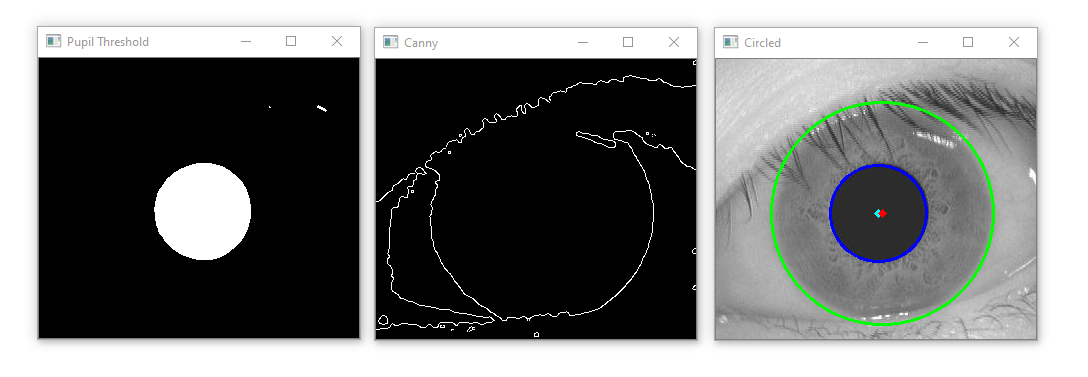
\includegraphics[width=1.0\textwidth]{hough.png}
  \caption{Esito dell'applicazione della funzione \texttt{cv2.HoughCircles}}
\end{figure}

\emergencystretch 5em%

Le funzioni \texttt{pupil\_recognition} e \texttt{iris\_recognition} presenti in \texttt{preprocessing.py}, ovvero le funzioni che si occupano di richiamare tutte le varie tecniche di elaborazione dell’immagine, terminano con l’Hough Circles Transform e quindi restituiscono in output i  valori di centro e raggio del cerchio trovato, tali valori verranno poi utilizzati nella successiva fase di segmentazione. Nel caso in cui invece non vengano trovati cerchi, oppure ne vengano trovati più di uno per iride e pupilla, l’immagine causa dei problemi viene scartata, quindi non sarà più considerata nell’insieme di immagini di training in quanto non potrà essere segmentata.
